\section{Vilpellet's method, step by step}\label{sec:method}

This section follows his reference inference script~\cite{vilpellet2025code}, which our rewrite
in \texttt{phases.py} reproduces bit for bit: features, Viterbi path and final labels coincide on
three real flights (\texttt{test\_note.py}). Every window counts fixes; on a 1-Hz track a fix is a
second.

\subsection{Local frame and smoothing}\label{sec:frame}

The method works on one piece of flight at a time, fixes in order. Latitude, longitude and GNSS
height become east, north and up coordinates $(e_k,n_k,u_k)$ in metres, in a frame tangent to the
Earth at the first fix of the piece (WGS84). Each coordinate is then smoothed with Gaussian
weights over six consecutive fixes, $k-3$ to $k+2$, with a standard deviation of one fix; the first
three and the last two fixes of a piece have no smoothed value. The third coordinate is the height
above the plane tangent at the first fix, which falls below the altitude by about $d^2/2R$ at a
distance $d$ from that fix: 785~m at 100~km. Its rate of change is the climb rate minus
$(d/R)\,\dot d$, with $\dot d$ the speed away from the first fix: 0.16~m/s less for a glide at
10~m/s, 100~km out (Section~\ref{sec:keep}).

\subsection{Turn and climb rate}\label{sec:turn}

The heading of the step from fix $k$ to fix $k+1$ is $\varphi_k=\operatorname{atan2}(n_{k+1}-n_k,\
e_{k+1}-e_k)$, and the \emph{turn} at fix $k$ is the change of heading, brought into $[-\pi,\pi)$
(Figure~\ref{fig:turn}):
\begin{equation}\label{eq:turn}
  \theta_k = \bigl((\varphi_k-\varphi_{k-1}+\pi) \bmod 2\pi\bigr)-\pi ,
\end{equation}
positive when the pilot turns left, anticlockwise seen from above. The turn is then averaged over
six fixes, $k-3$ to $k+2$. The code calls it \texttt{radius\_curvature} and the paper a curvature
angle; it is an angle per fix. A pilot circling once in 26~s turns by
$2\pi/26\approx0.24$~rad per fix. The climb rate is $v_{z,k}=(u_k-u_{k-1})/(t_k-t_{k-1})$, on the
smoothed height.

\begin{figure}
\centering
\begin{tikzpicture}[x=1cm,y=1cm]
  \coordinate (a) at (0,0); \coordinate (b) at (3,0.9); \coordinate (c) at (5.2,2.9);
  \draw[ink, line width=1pt, ->] (a) -- (b);
  \draw[ink, line width=1pt, ->] (b) -- (c);
  \draw[muted, densely dashed] (b) -- ($(b)!-1!(a)$);
  \foreach \p/\n in {a/{k-1}, b/k, c/{k+1}} \fill[ink] (\p) circle (2pt);
  \node[lbl, below] at (a) {fix $k-1$};
  \node[lbl, below right] at (b) {fix $k$};
  \node[lbl, above left] at (c) {fix $k+1$};
  \draw[transition, line width=0.9pt, ->] ($(b)+(16.7:1.3)$) arc (16.7:42.3:1.3);
  \node[lbl, transition] at ($(b)+(30:1.65)$) {$\theta_k$};
  \draw[ink2] (a) -- ++(1.3,0);
  \draw[ink2, ->] ($(a)+(1.1,0)$) arc (0:16.7:1.1);
  \node[lbl] at ($(a)+(1.75,-0.25)$) {$\varphi_{k-1}$};
  \node[note, anchor=west, align=left] at (6.2,1.4) {$\varphi$: heading of a step, from east, anticlockwise\\$\theta_k=\varphi_k-\varphi_{k-1}$: positive here, a left turn};
\end{tikzpicture}
\caption{The turn at fix $k$ is the angle between the step that arrives at the fix and the step that
leaves it.}
\label{fig:turn}
\end{figure}

\subsection{Three yes/no features}\label{sec:features}

Each fix $k$ looks at the 30 fixes $W_k=\{k-15,\dots,k+14\}$ around it and answers three
questions:
\begin{align}
  \text{straight:}\quad S_k &= \ind\Bigl[\,\bigl|\{m\in W_k:\ |\theta_m|<\alpha\}\bigr| > 0.9\times30\,\Bigr], \label{eq:S}\\
  \text{rising:}\quad R_k &= \ind\Bigl[\,\tfrac{1}{30}\textstyle\sum_{m\in W_k} v_{z,m} > 0\,\Bigr], \label{eq:R}\\
  \text{one sign:}\quad O_k &= \ind\bigl[\,\text{at least 14 of the 15 largest $|\theta_m|$ in $W_k$ share one sign}\,\bigr]. \label{eq:O}
\end{align}
$S_k=1$ needs at least 28 of the 30 turns below $\alpha$; $R_k=1$ a positive mean climb rate;
$O_k=1$ a pilot who turns one way.
In a straight glide the turn wobbles around zero with a random sign; only the strongest turns of
the window tell whether the pilot circles one way, which is why~\eqref{eq:O} looks at the 15 largest
only. Near the ends of a piece the means use the fixes available, and the window of~\eqref{eq:O}
reflects the series. Table~\ref{tab:signatures} lists the answers each phase should give;
Figure~\ref{fig:window} counts them on one window in each phase of a synthetic flight, and
Figure~\ref{fig:features} shows them on 24 minutes of a real flight.

\begin{figure}
\centering
\animated{window}
\caption{\animmark The three features on a synthetic flight of eight minutes at 1~Hz: a glide at
10~m/s sinking at 1.2~m/s, a search that turns both ways, and a left-hand climb at 1.8~m/s, one
turn in 24~s, drifting with a wind of 2~m/s; 0.5~m of noise on every coordinate. Top: the 30
fixes of one window in each phase, centred on the open circle, with the track around them in
grey. Bottom: their smoothed turns, with the band $|\theta|<\alpha$ in grey and the 15 largest in
black, and the three answers. In the glide no turn leaves the band; in the search the largest
turns go both ways; in the climb all fifteen are left turns. The animation slides the window
along the flight and draws the features and the labels as it goes.}
\label{fig:window}
\end{figure}

\begin{table}
\centering
\small
\begin{tabular}{@{}l c c c l@{}}
\toprule
phase & straight $S$ & rising $R$ & one sign $O$ & why \\
\midrule
\textcolor{climb}{\textbf{climb}} & 0 & 1 & 1 & circles one way and rises \\
\textcolor{search}{\textbf{search}} & 0 & 0 or 1 & 0 & turns both ways, height about constant \\
\textcolor{transition}{\textbf{transition}} & 1 & 0 & 0 & straight, sinking \\
\bottomrule
\end{tabular}
\caption{The answers each phase should give~\cite{vilpellet2025}.}
\label{tab:signatures}
\end{table}

\begin{figure}
\centering
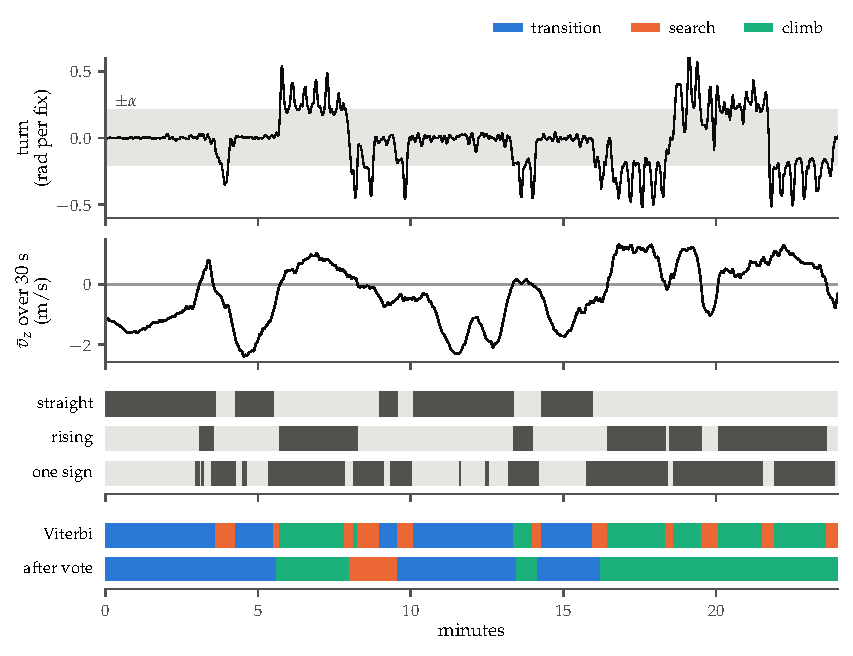
\includegraphics[width=\textwidth]{figures/features.pdf}
\caption{The features on 24 minutes of the flight of Figure~\ref{fig:flight}. From the top: the
smoothed turn, with the band $|\theta|<\alpha$ in grey; the climb rate averaged over 30~s; the
three features, dark when 1; the Viterbi path and the labels after the majority vote
(Section~\ref{sec:decoding}).}
\label{fig:features}
\end{figure}

\subsection{The straightness threshold}\label{sec:alpha}

$\alpha$ separates a turn from a wobble. Vilpellet reads it off the distribution of $|\theta|$ over
many fixes~\cite{vilpellet2026,vilpellet2025}: for paragliders and hang gliders the density decreases
from zero, first convex and then concave, and $\alpha$ is the inflection point between the two,
estimated with kernel estimates of the density and of its second derivative. He finds
$\alpha=0.2096$~rad per fix for paragliders and $0.1740$ for hang gliders ($0.10$ for sailplanes,
from a different rule). Figure~\ref{fig:alpha} shows where $\alpha$ falls on the turns of each
phase: 98\% of the transition fixes are below it, 66\% of the search fixes and 37\% of the climb
fixes.

\begin{figure}
\centering
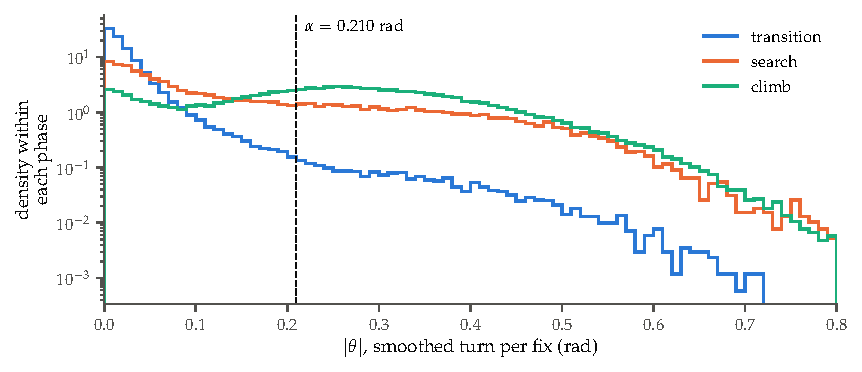
\includegraphics[width=\textwidth]{figures/turn_density.pdf}
\caption{Density of the smoothed $|\theta|$ in each phase, on 30 flights of the sample of
Section~\ref{sec:cadence}, labelled by the method; the dashed line is $\alpha$ for paragliders.}
\label{fig:alpha}
\end{figure}

\subsection{Symbols and emissions}\label{sec:emissions}

The three answers make one symbol, $x_k=4S_k+2R_k+O_k\in\{0,\dots,7\}$, and the model gives each
phase a probability for each of the eight symbols (Figure~\ref{fig:emissions}). A climb emits
almost only $(0,1,1)$, ``turning one way and rising''; a transition emits the straight symbols,
mostly $(1,0,0)$ and $(1,1,0)$; a search spreads over the other turning symbols, mostly $(0,1,0)$
and $(0,0,0)$, turning both ways with or without rising, and $(0,0,1)$, turning one way while
sinking. A straight symbol is practically impossible outside a transition, and $(0,1,1)$
practically impossible outside a climb. These symbols all but decide the phase: inside a glide a
single $(0,1,1)$ already turns the Viterbi path to climb, inside a search two in a row do, and the
majority vote of Section~\ref{sec:decoding} then removes such short runs. The HMM matters where
the symbols are ambiguous or change.

\begin{figure}
\centering
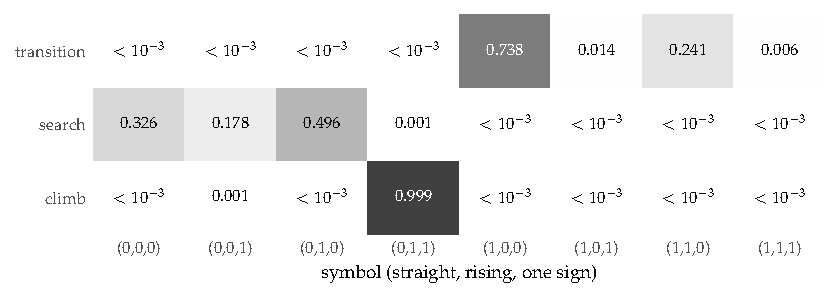
\includegraphics[width=\textwidth]{figures/emissions.pdf}
\caption{Emission probabilities $b_j(x)$ of the fitted model; each row sums to 1. Symbols are
written as (straight, rising, one sign).}
\label{fig:emissions}
\end{figure}

\subsection{Decoding and majority vote}\label{sec:decoding}

The Viterbi path~\eqref{eq:viterbi} is computed with $A$ of~\eqref{eq:A} and the initial
distribution
\[
  \nu=(0.0566,\ 0.9434,\ 6\times10^{-29}),
\]
with the scores divided by their sum at every fix; a tie goes to the phase that comes first in the
order \cl, \se, \tr. The initial probability of \tr\ is zero in practice: a piece never starts
in a transition.

The path still flickers at the changes of phase (Figure~\ref{fig:features}, ``Viterbi''). A
\emph{majority vote} follows: each fix takes the phase most frequent among the 90 fixes
$k-45,\dots,k+44$ of the path, a tie going to the phase that comes first. The vote removes the
flicker and also erases any run shorter than about 45~s, real or not.

\subsection{How the parameters were obtained}\label{sec:training}

The training script~\cite{vilpellet2025code} reads the 2019 paraglider flights from the take-offs
whose names contain Montlambert, Hilaire, Forclaz or André, keeps those with distinct
times, a mean step below 1.2~s and more than 3600 fixes, and runs five rounds of Baum--Welch from
initial values that encode Table~\ref{tab:signatures}. Each phase has one categorical law over the
eight symbols. The values in the inference script, which every later use applies unchanged, are
described there as ``a local max that is visually satisfying''. The same values serve hang gliders,
with only $\alpha$ changed. Section~\ref{sec:conflicts} lists what the code does differently from
what the paper describes.

\subsection{Which state is which}\label{sec:naming}

An HMM does not name its states (Section~\ref{sec:three}). The emissions do: the state that emits
$(0,1,1)$ is the climb and the one that emits straight symbols the transition. The training code
orders the states as thermalling, area-restricted search and commuting, consistently with the
emissions. The last line of the inference script, \texttt{regime\_map = \{0: "transition", 1:
"search", 2: "climb"\}}, swaps the first and the third. The emissions, and the climb rate,
straightness and turn sign measured in each state on five real flights~\cite{legacyguide}, show that
state 0 is the climb: the order is \cl, \se, \tr, as in this note.
